\begin{document}

\def\title{Worksheet 1}

\newcommand{\qitem}{\qpart\item}

\renewcommand{\labelenumi}{(\alph{enumi})} % change default enum format to (a)
\renewcommand{\theenumi}{(\alph{enumi})} % fix reference format accordingly.
\renewcommand{\labelenumii}{\roman{enumii}.} % second level labels.
\renewcommand{\theenumii}{\roman{enumii}.}

\maketitle

\vspace{0.5em}

\begin{qunlist}

% TODO: Add spacing for students to do problems between parts.

% \qns{An Introduction to Solving Differential Equations}
\qcontributor{Justin Yu}
\qcontributor{Taejin Hwang}

In this question, we will examine the process behind solving a 
first order differential equation and provide some motiviation for each step.

Consider the following first order differential equation:
\begin{align}
a \cdot \ddt{y(t)}{t} + b \cdot y(t) = c
\end{align}

We can divide the equation by $a$ to make the coefficient of $\ddt{y(t)}{t},$ one.
\begin{align}
\ddt{y(t)}{t} + \alpha \cdot y(t) = \beta
\end{align}

Our goal is to find a function $y(t)$ such that our differential equation 
is true for all values of $t.$
To do this, we use a guess and check approach.

\meta{
This question is supposed to walk through the process of solving a first order 
differential equation. While students may be familiar with the process, this 
question was made to motivate each step of the solving process.
}

\begin{enumerate}

\qitem Can you think of a function where $\ddt{y(t)}{t} = y(t)$ for all $t$?

\sol{
It can be seen either through inspection or integration that $y(t) = e^t.$
}

\qitem Now, how can you modify the function above to solve 
$\ddt{y(t)}{t} + \alpha y(t) = 0$?
This equation is known as the homogenous equation.

\sol{
We can notice that if $y(t) = e^{rt},$ then $\ddt{y(t)}{t} = re^{rt}.$
Therefore if we subtract $\alpha y(t),$ we get $\ddt{y(t)}{t} = -\alpha y(t).$ 
It follows by picking $r = -\alpha$ that $y(t) = e^{-\alpha t}$ 
satisfies our differential equation.
}

\end{enumerate}

You might notice that the solution above is not unique.
This is the reason a differential equation will often come 
with an initial condition such as $y(0) = 2$.

\begin{enumerate}[resume]

\qitem Try using this initial condition to solve for a 
unique solution to the differential equation above.

\meta{
Students may try plugging in $t = 0$ and arrive at a contradiction that $1 = 2.$
You may want to emphasize that $y(t) = e^{-\alpha t}$ isn't unique since 
$y(t) = Ke^{-\alpha t}$ works for any nonzero choice of $K \in \mathbb{R}.$

}

\sol{
Notice that our solution isn't unique since $y(t) = Ke^{-\alpha t}$ 
satisfies our differential equation for any nonzero choice of $K.$
Plugging in $t = 0,$ we get $y(0) = K = 2,$ so our solution is
$y(t) = 2 e^{-\alpha t}.$
}

\qitem Now, let's try solving our original equation:
\begin{align}
    \ddt{y(t)}{t} + \alpha y(t) = \beta
\end{align}
To do this, we will use a change of variables.
Let $\widetilde{y}(t) = y(t) - \frac{\beta}{\alpha}$.

\begin{enumerate}

\qitem Try writing the original equation as a differential 
equation in terms of $\widetilde{y}(t)$.

\sol{
Since $y(t) = \widetilde{y}(t) + \beta / \alpha, 
\ddt{y(t)}{t} = \ddt{\widetilde{y}(t)}{t}.$ 

Substituting these values, 
we see that $\ddt{\widetilde{y}(t)}{t} + \alpha \widetilde{y}(t) + \beta = \beta$
or $\ddt{\widetilde{y}(t)}{t} + \alpha \widetilde{y}(t) = 0.$
}

\qitem Does this equation look familiar? How can you solve this equation?

\sol{
This is the homogenous equation in terms of $\widetilde{y}(t)!$ \\
So by parts (b) and (c), our solution is $\widetilde{y}(t) = Ke^{-\alpha t}.$	
}


\qitem What is the final solution $y(t)$? Assume $y(0)$ is given.

\sol{
Converting back to $y(t),$ our solution is $y(t) = Ke^{-\alpha t} + \beta / \alpha.$
Plugging in $t = 0,$ we get $y(0) = K + \beta / \alpha$ or $K = y(0) - \beta / \alpha.$
Our final solution is $y(t) = y(0) e^{-\alpha t} + \beta / \alpha (1 - e^{-\alpha t}).$
}

\end{enumerate}

\end{enumerate}

To recap, given a first order differential equation $\ddt{y(t)}{t} + \alpha y(t) = \beta$, the solution is:
\begin{align}
    y(t) = y(0) e^{-\alpha t} + \frac{\beta}{\alpha} (1 - e^{-\alpha t})
\end{align}

\meta{
You can explain that $y(0)e^{-\alpha t}$ is the decaying exponential
of the initial condition, while \\ $\frac{\beta}{\alpha} (1 - e^{-\alpha t})$ represents
the growth of the steady state response.
}

Another form you might find useful is the steady state form:
\begin{align}
    y(t) = y(\infty) + (y(0) - y(\infty)) e^{-\alpha t}
\end{align}

\meta{
The second equation can be broken down into $y(\infty)$ which is the steady state
and $[y(0) - y(\infty)] e^{-\alpha t}$ which is the decaying exponential
of the initial state, from the steady state response.
}


% \newpage

% Authors: Justin Yu, Taejin Hwang
% Email: justinvyu@berkeley.edu, taejin@berkeley.edu

\qns{Non-homogeneous Differential Equations}

\meta {
	Prereqs: Solving a first-order homogeneous differential equation. 
}

Ordinary differential equations play a key role in modeling physical and electrical systems.
It was shown in lecture and in homework that for a first-order, constant coefficient ordinary differential equation,

\begin{equation} \label{eq:h}
\ddt{}{t} x(t) = \lambda x(t)
\end{equation}

with initial condition $x(0) = x_0,$ the particular solution to the equation, $x_p(t),$ was uniquely determined as:
\begin{equation} \label{eq:hs}
x_p(t) = x_0 e^{\lambda t}
\end{equation}

For the purposes of this question, we will look at the case in which we have a constant on the right hand side.
This is referred to as a \textbf{non-homogeneous differential equation}.

Now consider the following non-homogeneous differential equation with initial condition $x(0) = x_0$:
\begin{equation} \label{eq:nh}
    \ddt{}{t} x(t)  = \alpha x(t) + \beta, \ \forall t \geq 0
\end{equation}

\begin{enumerate}
\qitem To solve this, we want to come up with a change of variables $\widetilde{x}(t)$ such that $\frac{d}{dt} \widetilde{x}(t) = \alpha \widetilde{x}(t)$. 

\textbf{Write out $\widetilde{x}(t)$ in terms of $x(t)$.} \\
\sol {
	We want our change of variables to satisfy two conditions:
	\begin{align*}
		\frac{d}{dt} \widetilde{x}(t) = \frac{d}{dt} x(t) \\
		\alpha \widetilde{x}(t) = \alpha x(t) + \beta
	\end{align*}
	These two conditions are satisfied by
	\begin{align*}
		\widetilde{x}(t) = x(t) + \frac{\beta}{\alpha}
	\end{align*}
}

\qitem Using the change of variables you just derived, \textbf{write equation (\ref{eq:nh}) and the initial condition of the differential equation in terms of $\widetilde{x}(t)$.} \\
Don't forget about the initial condition!

\ws{
	\vspace{75px}
}

\meta {
  Hint to students: Try calculating $\ddt{}{t}x(t)$ and see if you can substitute.
}

\sol{
  Since $\alpha \widetilde{x}(t) = \alpha x(t) + \beta,$ and $\ddt{}{t}x(t) = \ddt{}{t}\widetilde{x}(t).$ 
  Substituting these values, we see that $\ddt{}{t}\widetilde{x}(t) = \alpha \widetilde{x}(t)$
  The initial condition will be $\widetilde{x}(0) = x(0) + \beta / \alpha.$ 
}

\qitem \textbf{Does this equation look familiar? How can you solve this equation?}

\ws{
	\vspace{75px}
}

\sol{
  This is the homogeneous equation \eqref{eq:h} in terms of $\widetilde{x}(t)!$ 
  Since this is a homogeneous differential equation, in terms of $\widetilde{x}(t),$ using the particular solution $x_p(t)$ provided above, our solution is $\widetilde{x}_{p}(t) = \widetilde{x}_{0} e^{\alpha t}.$
}

\qitem \textbf{What is the final solution $x(t)$?} Assume that $x(0) = x_0$ is a given constant.

\ws{
	\vspace{75px}
}

\sol{
  Converting back to $x(t),$ our solution is $x(t) = \widetilde{x}_{0} e^{\alpha t} - \beta / \alpha.$
  Then substituting the initial condition in, our final solution is $x(t) = x(0) e^{\alpha t} - \frac{\beta}{\alpha} (1 - e^{\alpha t}). $
}

\end{enumerate}

To recap, given a first order differential equation $\ddt{}{t} x(t) = \alpha x(t) + \beta$, the solution will be determined as:
\begin{equation} \label{eq:nhs}
    x(t) = x(0) e^{\alpha t} - \frac{\beta}{\alpha} (1 - e^{\alpha t})
\end{equation}

\meta{
  You can explain that $x(0)e^{\alpha t}$ is the decaying exponential of the initial condition, while \\ $\frac{\beta}{\alpha} (1 - e^{\alpha t})$ represents the growth of the steady state response.
}

% Another form you might find useful is the steady state form:
% \begin{align}
%     x(t) = y(\infty) + (x(0) - y(\infty)) e^{-\alpha t}
% \end{align}

% \meta{
% The second equation can be broken down into $y(\infty) = \beta / \alpha$ which is the steady state, and

% $[x(0) - y(\infty)] e^{-\alpha t}$ which is the decaying exponential of the initial state, from the steady state response.
% }

% \begin{enumerate}[resume]

% \qitem Show that $x_{p}$(t) does indeed satisfy the differential equation \eqref{eqn:odeinput}. \\
% \textit{Hint: Is there anything you can pull out of the integral to make sure there are no terms with $t$ in the integrand?}

% \meta{
%   The second line of work uses the product rule of derivatives combined with the Second Fundamental Theorem of Calculus.
% }

% \sol{
% To show that $x_{p}$(t) satisfies equation \eqref{eqn:odeinput}, we have to show that it satisfies the the general differential equation and the initial condition. \\
% For the general differential equation, we will show that $\ddt{x_p(t)}{t} = \lambda x_p(t) + u(t)$.
% $$\ddt{x_p(t)}{t} = \lambda x_0 e^{\lambda t} + \ddt{}{t}(e^{\lambda t} \int_0^t \! u(\tau)e^{-\lambda \tau} \, d\tau)$$
% $$\ddt{x_p(t)}{t} = \lambda x_0 e^{\lambda t} + \lambda e^{\lambda t} \int_0^t \! u(\tau)e^{-\lambda \tau} \, d\tau +  e^{\lambda t}u(t)e^{-\lambda t} = \lambda x_p(t) + u(t)$$
% We also have to show that $x_p(0) = x_0$:
% $$x_p(0) = x_0e^{\lambda \cdot 0} + \int_0^0 \! u(\tau)e^{-\lambda \tau} \, d\tau = x_0 + 0 = x_0$$
% }

% \end{enumerate}

We will now take this insight and apply it to the process of charging up a capacitor.
\newline

Consider the circuit below, assume that when $t\leq 0$, the capacitor has no charge stored $(V_{C}(t=0) = 0)$.
At $t=0$, the switch closes. Assume that $V_s=\SI{5}{\volt}$, $R=\SI{100}{\ohm}$, and $C=\SI{10}{\micro\farad}$.

\begin{figure}[H]
	\begin{centering}
		\begin{circuitikz}
			\draw (0, 4)
			to[V =$V_s$] (0, 0);
			\draw (0, 4)
			to[switch,l^=\mbox{$t = 0$}](4,4)
			(4,4) to[R = $R$,v=$V_R(t)$,i>^=$i_R(t)$] (7,4)	
			to [short] (9,4)
			to[C = $C$, v=$V_C(t)$,i>^=$i_C(t)$] (9,0)
			to [short] (0,0);
		\end{circuitikz}
		\caption{\label{fig:circuit}RC Circuit with Voltage Source}
	\end{centering}
\end{figure}

\meta{
	The rest of this problem is meant to be an introduction to transient analysis of circuits.
	Make sure students fully understand the concepts presented (how to get a differential equation from the circuit, how to solve the equation, and the physical intuition of what is happening in the circuit - charging up a capacitor) before moving on.
}
\begin{enumerate}[resume]

\qitem \textbf{Write out the KCL equations associated with the circuit when the switch is closed.}

\ws{\vspace{75px}}

\meta{
	To simplify your circuit analysis, mark the negative end of the voltage source as ground.
}

\sol{
\begin{align*}
\intertext{We denote the voltage to the left of resistor to be $V_s.$}
\intertext{By KCL, the current through the resistor } i_R = i_{\text{C}}.
\intertext{Ohm's law tells us that } i_R = \frac{V_s - V_{C}}{R}
\intertext{The voltage-current relationship of a capacitor tells us that }i_\text{C} = C\ddt{V_{C}}{t}
\intertext{Therefore, } \frac{V_s - V_{C}}{R} = C \ddt{V_{C}}{t}
\end{align*}
}

\qitem \textbf{Write out the differential equation for $V_{\text{C}}(t)$ after the switch closes.}

\ws{
\vspace{75px}
}

\meta{
	If students are confused about how to get started, point them to equation \eqref{eq:nh} in problem 1 as a template.
	Which KCL equation from part (a) of this problem resembles a first order differential equation (i.e. which one has a differential term)?
}

\sol{
\begin{align*}
\intertext{From the previous problem we know that when the switch is closed,}
\frac{V_{\text{s}}- V_{C}}{R} = C\frac{dV_{C}}{dt} \\
\intertext{Thus we obtain}
\ddt{V_{C}}{t} + \frac{V_{C}}{RC} = \frac{V_{\text{S}}}{RC}
\end{align*}
}

\sol{
No charge is on the capacitor before time $t=0$. Using $q=VC$, we know that $V_{C}=\SI{0}{\volt}$ before $t=0$.
At $t=0$, the switch closes. Since voltage across the capacitor cannot change instantaneously, $V_{C}(t=0)=0.$
As $t$ goes to infinity, the capacitor will become fully charged and the current goes to zero.
Therefore, the voltage of the capacitor equals the voltage source: $V_{C}(t \to \infty) = V_{\text{S}}.$
}

\qitem \textbf{Using the initial conditions found in the previous parts, find an expression for
$V_{\text{C}}(t)$ in terms of $V_{\text{s}}$, $R$, and $C$.}

\meta{
	You can point at equation \eqref{eq:nhs} and find the appropriate values of $\alpha$ and $\beta,$ 
	but let them know that they are still expected to know how to do the process below. 	
}


\sol{
	To find an expression for $V_{out}(t)$:
	\[V_c(t)=V_{out}(t)\]
	\[\frac{dV_{out}(t)}{dt}+\frac{1}{RC}V_{out}(t)=\frac{V_{S}}{RC}\]

	Using substitution of variables:
	\[x(t) = V_{out}(t)-V_{S}\]
	\[V_{out}(t)=x(t)+V_{S}\]
	\[\frac{dV_{out}(t)}{dt}=\frac{dx(t)}{dt}\]
	\[\frac{dx(t)}{dt}+\frac{1}{RC}x(t)=0\]
	\[x(t)=Ae^{-\frac{t}{RC}}\]

	Now substituting back to find $V_{out}$:
	\[V_{out}(t)=V_{S}+Ae^{-\frac{t}{RC}}\]

	Using our initial condition:
	\[V_{out}(0)=0=V_{S}+A\]
	\[A=-V_{S}\]
	\[V_{out}(t)=V_{S}\left(1-e^{-\frac{t}{RC}}\right)\]
	\[V_c(t) = V_S(1 - e^{-\frac{t}{\tau}}) \text{ where } \tau = RC\]
}

\meta{
	Using this equation, you can see that the steady state voltage of the capacitor is $V_S$. As time goes to $\infty$, the $-V_S e^{-t/\tau})$ term (called the \textbf{transient response}) goes to 0, so the voltage approaches $V_S$ as the charges.
}

\end{enumerate}
\newpage

% Authors: Naomi Sagan, Justin Yu

\qns{RC Transistor Model}

Consider a single CMOS inverter with a voltage input, except there is some resistance between the voltage source and the gates of the transistors.

\vspace{-1em}

\begin{center}
    \begin{figure}[H]
	\begin{centering}
		\begin{circuitikz}[scale=0.8]
				\draw (-1,4) 
				to [V=$V_{in}$](-1, 2) to (-1,2) node[ground]{}; 
				\draw (4,5) node[pmos, emptycircle](pm){} ;
				\draw (4,3) node[nmos, ](nm){} ;
				\draw (-1,4) to [R = $R$] (2,4) to [short] (2,5)
				to (pm.gate);
				\draw (pm.source) to [short, -*] (4,6) node[above]{$V_{DD}$};;
				\draw (pm.drain) to (nm.drain);
				\draw (2,4) to [short] (2, 3) to (nm.gate);
				\draw (nm.source) to (4,2) node[ground]{};
				\draw (4,4) [short] to [short, -*] (5,4) node[right]{$V_{out}$};
		\end{circuitikz}
		\caption{\label{fig:circuit}CMOS Inverter with Resistance}
	\end{centering}
\end{figure}
\end{center}

\vspace{-4em}

\begin{enumerate}

\qitem First, let's introduce a way to model CMOS transistors.
A transistor can be modeled with a capacitor between the gate $G$ and source $S$, an internal resistance, and a voltage-controlled switch between drain $D$ and $S$.

\textbf{Using the NMOS and PMOS transistor models below, redraw the inverter as a simple RC circuit.}

\noindent
\begin{figure}[ht]
\centering
\begin{subfigure}{.48\textwidth}
\flushleft
\begin{subfigure}{.3\textwidth}
\centering
\begin{circuitikz}[american] 
\draw (0, 0) node[pmos] (nmos) {};
\draw (nmos.G) node[left]{$G$};
\draw (nmos.S) node[left]{$S$};
\draw (nmos.D) node[left]{$D$};
\end{circuitikz}
\end{subfigure}
\centering
\begin{subfigure}{.2\textwidth}
\flushright\begin{circuitikz}[american] 
\draw (0, 1) node[ocirc]{} node[above]{$G$}
      to[short] (0, -1)
      to[C = $C_{GS}$, v=$V_{GS}$] (2, -1);
\draw (2, -1) node[ocirc]{} node[below]{$S$}
      to[switch, l_=$V_{SG} \geq |V_{tp}|$] (2, 1)
      to[R=$R_{on_, P}$] (2, 2.2)
      to[short] (2, 3.4)
      node[ocirc]{} node[above]{$D$} (2, 4);
\end{circuitikz}
\end{subfigure}
\caption{PMOS Transistor Model}
\end{subfigure}
\begin{subfigure}{0.48\textwidth}
\flushleft
\begin{subfigure}{.3\textwidth}
\centering
\begin{circuitikz}[american] 
\draw (0, 0) node[nmos] (nmos) {};
\draw (nmos.G) node[left]{$G$};
\draw (nmos.S) node[left]{$S$};
\draw (nmos.D) node[left]{$D$};
\end{circuitikz}
\end{subfigure}
\centering
\begin{subfigure}{.2\textwidth}
\flushright
\begin{circuitikz}[american] 
\draw (0, 1) node[ocirc]{} node[above]{$G$}
      to[short] (0, -1)
      to[C = $C_{GS}$, v=$V_{GS}$] (2, -1);
\draw (2, -1) node[ocirc]{} node[below]{$S$}
      to[switch, l_=$V_{GS} \geq V_{tn}$] (2, 1)
      to[R=$R_{on_, N}$] (2, 2.2)
      to[short] (2, 3.4)
      node[ocirc]{} node[above]{$D$};
% \draw (0, 0) to[open, v=$V_{GS}$] (1, -1);
\end{circuitikz}
\end{subfigure}
\caption{NMOS Transistor Model}
\end{subfigure}
\end{figure}

% \begin{figure}
% \centering
% \begin{subfigure}{.2\textwidth}
% \centering
% \begin{circuitikz}[american] 
% \draw (0, 0) node[nmos] (nmos) {};
% \draw (nmos.G) node[left]{$G$};
% \draw (nmos.S) node[left]{$S$};
% \draw (nmos.D) node[left]{$D$};
% \end{circuitikz}
% \end{subfigure}
% \begin{subfigure}{.2\textwidth}
% \centering
% \begin{circuitikz}[american] 
% \draw (0, 1) node[ocirc]{} node[above]{$G$}
%       to[short] (0, -1)
%       to[C = $C_{GS}$, v=$V_{GS}$] (2, -1);
% \draw (2, -1) node[ocirc]{} node[below]{$S$}
%       to[switch, l_=$V_{GS} \geq V_{tn}$] (2, 1)
%       to[R=$R_{on_, N}$] (2, 2.2)
%       to[short] (2, 3.4)
%       node[ocirc]{} node[above]{$D$};
% % \draw (0, 0) to[open, v=$V_{GS}$] (1, -1);
% \end{circuitikz}
% \end{subfigure}
% \caption{NMOS Transistor Model}
% \end{figure}

% \centering
% \begin{circuitikz}[american] 
% \draw (0, 0) node[ocirc]{} node[above]{$G$};
% \draw (1, -1) node[ocirc]{} node[below]{$S$} to[switch] (1, 1) node[ocirc]{} node[above]{$D$};
% \draw (0, 0) to[open, v=$V_{GS}$] (1, -1);
% \end{circuitikz}
% % \caption{$V_{GS} > V_{th, N}$}

\newpage

\sol{}

\qitem
We want to analyze the behavior of the inverter by solving for the gate voltage $V_{GS}$ \textit{of the bottom NMOS transistor} as a function of time. \textbf{Using KCL or KVL, write out a differential equation for $V_{GS}$.}

\ws{\vspace{8em}}

\sol{}

\qitem 
Assume that $V_{in}$ has been low ($V_{in} = 0$) for a long time and switches to high ($V_{in} = V_{DD}$) at time $t = 0$. \textbf{Solve for $V_{GS}(t)$ using the differential equation from the last part and the above initial condition.}

\ws{\vspace{8em}}

\sol{}
\meta{}

\end{enumerate} % TODO: make this a MOSFET + RC problem
\newpage

% % Authors: Shreyas Krishnaswamy, Naomi Sagan, Taejin Hwang
% Email: shrekris@berkeley.edu, naomi.sagan@berkeley.edu, taejin@berkeley.edu

\qns{RC Circuits with Non-Constant Inputs}

In an earlier question we looked at a way to solve differential equations with a constant $\beta.$
\par

We will now generalize this to an input, $u(t),$ which is an function independent of $x(t)$.
It was shown in homework that if we had the differential equation
\begin{equation} \label{eqn:odeinput}
  \ddt{}{t} x(t) = \lambda x(t) + u(t)
\end{equation}

With an initial condition $x(0) = x_0,$ the solution was uniquely determined by:
\begin{equation} \label{eqn:odesol}
    x_{p}(t) = x_{0}e^{\lambda{}t} + \int_0^t \! u(\tau{})e^{\lambda{}(t - \tau{})} \, d\tau{}
\end{equation}

\begin{enumerate}

\qitem Show that $x_{p}$(t) does indeed satisfy the differential equation \eqref{eqn:odeinput}. \\
\textit{Hint: Is there anything you can pull out of the integral to make sure there are no terms with $t$ in the integrand?}

\meta{
  The second line of work uses the product rule of derivatives combined with the Second Fundamental Theorem of Calculus.
}

\sol{
To show that $x_{p}$(t) satisfies equation \eqref{eqn:odeinput}, we have to show that it satisfies the the general differential equation and the initial condition. \\
For the general differential equation, we will show that $\ddt{x_p(t)}{t} = \lambda x_p(t) + u(t)$.
$$\ddt{x_p(t)}{t} = \lambda x_0 e^{\lambda t} + \ddt{}{t}(e^{\lambda t} \int_0^t \! u(\tau)e^{-\lambda \tau} \, d\tau)$$
$$\ddt{x_p(t)}{t} = \lambda x_0 e^{\lambda t} + \lambda e^{\lambda t} \int_0^t \! u(\tau)e^{-\lambda \tau} \, d\tau +  e^{\lambda t}u(t)e^{-\lambda t} = \lambda x_p(t) + u(t)$$
We also have to show that $x_p(0) = x_0$:
$$x_p(0) = x_0e^{\lambda \cdot 0} + \int_0^0 \! u(\tau)e^{-\lambda \tau} \, d\tau = x_0 + 0 = x_0$$
}

\end{enumerate}

We will now take this insight and apply it to an RC circuit with non-constant input. Suppose $V_{c}(0) = 5V$.

\begin{figure}[H]
 \begin{figure}[H]
	\begin{centering}
		\begin{circuitikz}
			\draw (0, 2)
			to[V = $u(t)$] (0, 0)
			to node[ground]{} (0, 0);
			\draw (0, 2)
			to[R = $R$] (2.5, 2)
			to node[circ, label={$V_{C}(t)$}]{} (2.5, 2);
			\draw (2.5, 2)
			to[C = $C$] (2.5, 0)
			to node[ground]{} (2.5, 0);
		\end{circuitikz}
		\caption{\label{fig:circuit}RC Circuit with Voltage Source}
	\end{centering}
\end{figure}

\end{figure}
Let $u(t) = cos(\omega{}t)$, where $\omega{}$ denotes the frequency of the cosine wave.

\begin{enumerate}[resume]

\qitem Write out the KCL equations combined with Ohm's Law and the voltage-current relation of a capacitor.

\sol{
For this solution, we labeled the currents in the circuit as the following: \\
\begin{figure}[H]
 \begin{figure}[H]
	\begin{centering}
		\begin{circuitikz}
			\draw (0, 2)
			to[V = $u(t)$] (0, 0)
			to node[ground]{} (0, 0);
			\draw (2.5, 2)
			to node[circ, label={$V_{C}(t)$}]{} (2.5, 2)
			to[R = $R$, i^<=$i_R$] (0, 2);
			\draw (2.5, 2)
			to[C = $C$, i=$i_C$] (2.5, 0)
			to node[ground]{} (2.5, 0);
		\end{circuitikz}
		\caption{\label{fig:circuit}RC Circuit with Voltage Source}
	\end{centering}
\end{figure}

\end{figure}
Applying the KCL at the $V_c$ node, we get $I_R(t) = I_C(t)$
Substituting resistor and capacitor IV relationships, we have
  $$\frac{u(t) - V_c(t)}{R} = C \ddt{V_c(t)}{t}$$
}

\qitem Show that your equation above can be put into the form of equation \eqref{eqn:odeinput}.

\sol{
Rearranging terms in out KCL equation,
  $$\ddt{V_c(t)}{t} = - \frac{V_c(t)}{RC} + \frac{cos(\omega t)}{RC}$$
}

\qitem In this case, what are the values of $\lambda{}$, $x(t)$, $u(t),$ and $x_{0}$?

\meta{
  We wrote this question to make sure students are familiar with type-checking. 
}

\sol{
  $\lambda$ is $-\frac{1}{RC}, \, x(t)$ is $V_c(t)$, $u(t)$ is $\frac{\cos (\omega t)}{RC}$ and our initial condition $x_{0} = V_c(0) = 5V$ 
}

\qitem Using this particular solution, write out an expression for $V_{c}(t)$.

\meta {
  Make sure students know that they're supposed to write out an integral expression, and not actually solve the integral.
  Also, we used exp notation here since the fraction of the integral looked too small to distinguish between $t$ and $\tau.$
}

\sol{
  Plugging our values of $\lambda{}$, $x(t)$, $u(t),$ and $x_{0}$ into equation \eqref{eqn:odesol}, we get
    $$V_c(t) = 5e^{-\frac{t}{RC}} + \int_0^t \! \frac{cos(\omega \tau)}{RC} \text{exp}(-\frac{t - \tau}{RC}) \, d\tau$$
}

\qitem OPTIONAL: What is the closed form solution to the voltage across the capacitor, $V_{c}(t)$.\\
\textit{Hint:} $\int \! e^{at}cos(bt) \, dt = \frac{e^{at} (a \cdot cos(bt) + b \cdot sin(bt))}{a^2 + b^2} + C$

\meta{
  This is an extremely nasty integral. The purpose of the question obviously isn't to understand the nastiness of the integral.
  Most of this problem is done once they realize what the values of $a$ and $b$ are in the hint.
  The main purpose of this part is to show students how difficult transient analysis can get, and should foreshadow phasors.  
}

\sol{
  Rearranging terms in our expression for $V_{c}(t)$, we get 
  $$V_c(t) = 5e^{-\frac{t}{RC}} + \frac{e^{-\frac{t}{RC}}}{RC} \int_0^t \! cos(\omega \tau) e^{\frac{\tau}{RC}} \, d\tau$$
  Using the hint above to evaluate the integral (with $a = \frac{1}{RC}$ and $b = \omega$):
  $$V_c(t) = 5e^{-\frac{t}{RC}} + \frac{e^{-\frac{t}{RC}}}{RC} \cdot \frac{e^{\frac{t}{RC}} (\frac{1}{RC} \cdot cos(\omega t) + \omega \cdot sin(\omega t)) - \frac{e^{0}}{RC} \cos(\omega \cdot 0)}{\frac{1}{R^2C^2} + \omega^2}$$
  Simplifying slightly,
  $$V_c(t) = 5e^{-\frac{t}{RC}} + \frac{1}{(RC)^2} \frac{cos(\omega t) + \omega RC \cdot sin(\omega t) - e^{-\frac{t}{RC}}}{\frac{1}{(RC)^2} + \omega^2}$$
  So it follows that,
  $$V_c(t) = 5e^{-\frac{t}{RC}} + \frac{cos(\omega t) + \omega RC \cdot sin(\omega t) - e^{-\frac{t}{RC}}}{1 + (\omega RC)^2}$$
}

\end{enumerate}
 % TODO: merge this into first problem
% \newpage

% Author: Yannan Tuo, Varsha Ramakrishnan, Taejin Hwang
% Email: ytuo@berkeley.edu, vio@berkeley.edu, taejin@berkeley.edu
% Edited Lydia Lee, Spring 2019
% lydia.lee@berkeley.edu
% Edited: Justin Yu, Spring 2020
% justinvyu@berkeley.edu

\qns{Eigendecomposition and Change of Basis}

\meta{
  Please do a mini-lecture on change of basis similar to the opening paragraph of the change of coordinates question before doing this one.It is crucial that students understand change of basis, and how to convert from different bases first, before trying to understand eigendecomposition. It is up to you whether you want to mention the fact that all diagonalizable linear operators have a diagonal matrix representation given the correct choice of basis.
}

\textbf{Diagonal matrices}, matrices where all entries outside of the diagonal are zero, are often desirable since they are easy to analyze.
Determining properties such as rank and invertibility, are much simpler on a diagonal matrix as opposed to other non-diagonal matrices.
The process of \textbf{changing to a basis} in which the linear operator has a diagonal matrix representation is called \textbf{eigendecomposition} or \textbf{diagonalization.} You can think of eigendecomposition as a change of basis to one entirely made up of eigenvectors.

So what is a \textbf{change of basis}? Consider an arbitrary vector in $\mathbb{R}^2$: $\vec{x} = [ x_1 \text{ } x_2 ]^T$.
When we write a vector in this form, we are representing it as a linear combination of the \textit{standard basis} vectors for $\mathbb{R}^2$: $\vec{x} = x_1 \begin{bsmallmatrix} 1 \\ 0 \end{bsmallmatrix} + x_2 \begin{bsmallmatrix} 0 \\ 1 \end{bsmallmatrix}$. Naturally, $x_1$ and $x_2$ are the \textit{coordinates} of $\vec{x}$ in the standard basis (as you would refer to them if you graphed $\vec{x}$ on a Cartesian plane).

Now what if we wanted to represent that same vector in a different basis?
For example, say you wanted to represent the same vector $\vec{x}$ using the set of basis vectors $\vec{v_1}$ and $\vec{v_2}$.
This means that we need to find scalars $\alpha_1$ and $\alpha_2$ such that $\vec{x}$ can be written as a linear combination of these new basis vectors: $\vec{x} = \alpha_1 \vec{v_1} + \alpha_2 \vec{v_2}$.
To do this, we can just setup and solve a system of linear equations of the form:
$$\begin{bmatrix} \vec{v_1} & \vec{v_2} \end{bmatrix} \begin{bmatrix} \alpha_1 \\ \alpha_2 \end{bmatrix} = \begin{bmatrix} x_1 \\ x_2 \end{bmatrix}$$

In this problem, we'll investigate changing to and from the \textbf{eigenbasis} for the following matrix:

$$A = \begin{bmatrix}
2 & 2 \\
5 & -1
\end{bmatrix}$$

\begin{enumerate}

\qitem \textbf{Find $\lambda_1, \lambda_2$, the eigenvalues of $A$, ordered from largest to smallest.}
\ws{
\vspace{100px}
}

\meta {
  These first two parts are optional if students are comfortable with the process of finding eigenvalues and eigenspaces.
  It gives some concrete values that students can try out for the rest of the problem. If your students aren't convinced
  by $A = VDV^{-1}$, have them try out the concrete example with the numbers calculated in the first two parts.
}

\sol{
  \begin{align*}
    \text{det}(A - \lambda I) &= 0 \\
    (2 - \lambda) (-1 - \lambda) - 2(5) &= 0 \\
    \lambda^2 - \lambda - 12 &= 0 \\
    \implies \lambda_1 &= 4 \\
    \lambda_2 &= -3
  \end{align*}
}

\qitem \textbf{Find the eigenvectors $\vec{v_1}, \vec{v_2}$ corresponding to the eigenvalues.}

\ws{
\vspace{100px}
}

\sol{
  % \begin{bmatrix} 1 \\ 1 \end{bmatrix} \\ \begin{bmatrix} 1 \\ -1 \end{bmatrix}
  $$\vec{v_1} = \alpha \begin{bmatrix} 1 \\ 1 \end{bmatrix}$$
  $$\vec{v_2} = \beta \begin{bmatrix} -1 \\ -5/2 \end{bmatrix}$$
}

\end{enumerate}

With the eigenvectors we just found, define $V$ to be the matrix:
$$V = \begin{bmatrix}
\vec{v_1} & \vec{v_2}
\end{bmatrix}$$

\begin{enumerate}[resume]

\qitem Let $\widetilde{\vec{x}}$ be the coordinates of $\vec{x}$ in the eigenbasis. This means that for some arbitrary vector represented in the eigenbasis $\widetilde{\vec{x}} = \begin{bmatrix} \alpha_1 \\ \alpha_2 \end{bmatrix}$, the corresponding representation in standard coordinates is a linear combination of the columns of $V$: $\vec{x} = \alpha_1 \vec{v_1} + \alpha_2 \vec{v_2}$. \textbf{What is $\widetilde{\vec{x}}$ in terms of $V$ and $\vec{x}?$}

(\textit{Hint: Write $\vec{x}$ in terms of $V$ and $\tilde{\vec{x}}$, then go from there.})

\ws{\vspace{3em}}

\meta{
  The line $\alpha_1 \vec{v_1} + \alpha_2 \vec{v_2} = V \widetilde{\vec{x}}$ is not the most intuitive.
  It may require you showing on the board, why matrix vector multiplication can be seen as a linear combination of the columns.
}

\sol{
  $\vec{x} = \alpha_1 \vec{v_1} + \alpha_2 \vec{v_2} = V \widetilde{\vec{x}}.$ So it follows that $\widetilde{\vec{x}} = V^{-1} \vec{x}.$
}

\qitem It is often helpful to visualize the change of basis in a state diagram, where \textit{each arrow represents left-multiplying the variable it's coming out of by the corresponding matrix.} \textbf{Fill in the missing matrix operations in the state diagram based on your answer from the previous part.}

\ws {
  \begin{figure}[H]
    \centering
    \begin{tikzpicture}[node distance = 2cm, thick,every node/.style={inner sep=0.25em,outer sep=0.25em}]%
      \node (1) [circle,draw,minimum size=2em] {$\vec{x}$};
      \node (2) [circle,draw,right=of 1,minimum size=2em] {$\widetilde{\vec{x}}$};
      \draw[->] (1.45) -- node [rectangle,draw,midway,above,minimum size=2.5em] {} (2.135);
      \draw[->] (2.225) -- node [rectangle,draw,midway,below,minimum size=2.5em] {} (1.315);
    \end{tikzpicture}%
  \end{figure}
}

\meta {
  Not everyone finds this diagram the most intuitive, but it definitely helps a large percentage of students. Stress to students that it's always better to understand the intuitive meaning behind change of basis than to remember any particular change of basis formula. This intuitive meaning is bridging between coordinate systems, which can be visualized with this diagram.
}

\sol {
  \begin{figure}[H]
  \centering
  \begin{tikzpicture}[node distance = 2cm, thick,every node/.style={inner sep=0.25em,outer sep=0.25em}]%
    \node (1) [circle,draw,minimum size=2em] {$\vec{x}$};
    \node (2) [circle,draw,right=of 1,minimum size=2em] {$\widetilde{\vec{x}}$};
    \draw[->] (1.45) -- node [rectangle,draw,midway,above,minimum size=2.5em] {$V^{-1}$} (2.135);
    \draw[->] (2.225) -- node [rectangle,draw,midway,below,minimum size=2.5em] {$V$} (1.315);
  \end{tikzpicture}%
  \end{figure}
}


\qitem Now that we are able to switch back and forth between the coordinate systems, let's see how the linear transformation brought by $A$ can be viewed as a diagonal scaling transformation in the eigenbasis coordinate system.% Might be a bit confusing.

Let $\vec{y} = A \vec{x}$, and $\vec{x} = \alpha_1 \vec{v_1} + \alpha_2 \vec{v_2}$, using the same matrix $A$ and eigenvectors $\vec{v_1}, \vec{v_2}$ from before. Let $\widetilde{\vec{x}}$, $\widetilde{\vec{y}}$ be the coordinates of $\vec{x}$, $\vec{y}$ in the eigenbasis. \textbf{Find $\widetilde{\vec{x}}$ and $\widetilde{\vec{y}}$ in terms of $\alpha_1, \alpha_2, \lambda_1, \lambda_2$. What can we say about the relationship between $\widetilde{\vec{x}}$ and $\widetilde{\vec{y}}$?} % Might be confusing as to what the problem is asking compared to the next part.

(\textit{Hint}: Your answers shouldn't be in terms of the original $\vec{x}$ or $\vec{y}$.
 Use what you know about the coordinates of a vector in a certain basis; there is no need to invert any matrices or do any major computation.)

\ws {
  \vspace{100px}
}

\meta {
  Students may try to use what they found in the previous parts to multiply the vectors by $V^{-1}$. While this is technically right, make sure they understand what exactly
  that transformation is doing and why they don't need to do any matrix computation to find the coordinates of $\vec{y}$ in the eigenbasis.
}

\sol {
  $$\widetilde{\vec{x}} = \begin{bmatrix} \alpha_1 \\ \alpha_2 \end{bmatrix}$$

  \begin{align*}
    \vec{y} &= A \vec{x} \\
    &= A(\alpha_1 \vec{v_1} + \alpha_2 \vec{v_2}) \\
    &= \alpha_1 A \vec{v_1} + \alpha_2 A \vec{v_2} \\
    &= \alpha_1 \lambda_1 \vec{v_1} + \alpha_2 \lambda_2 \vec{v_2} \\
    \implies \widetilde{\vec{y}} &= \begin{bmatrix} \alpha_1 \lambda_1 \\ \alpha_2 \lambda_2 \end{bmatrix}
  \end{align*}

  This means that the matrix $D$ relating the two coordinates in the eigenbasis must be a diagonal scaling transformation, with the eigenvalues as the amount each dimension is scaled by.
}

\qitem \textbf{Find the matrix $D$ satisfying $\widetilde{\vec{y}} = D \widetilde{\vec{x}}$ in terms of $V$ and $A$.}

(\textit{Hint}: Start by writing $\vec{x}, \vec{y}$ in terms of $\widetilde{\vec{x}}$ and $\widetilde{\vec{y}}$. Refer to the state diagram from before.)

\ws{\vspace{120px}}

\meta {
  If students are comfortable with matrices representing linear transformations, you can explain this eigendecomposition as translating a linear transformation to and from the eigenbasis. For the diagonalization $A = VDV^{-1}$, left-multiplying an arbitrary vector $\vec{x}$ is equivalent to the following:

  \begin{align*}
    A \vec{x} &= VDV^{-1} \vec{x} \\
    &= VD \widetilde{\vec{x}} \\
    &= VD \begin{bmatrix} \alpha_1 \\ \alpha_2 \end{bmatrix} \\
    &= V \begin{bmatrix} \alpha_1 \lambda_1 \\ \alpha_2 \lambda_2 \end{bmatrix} \\
    &= V \widetilde{\vec{y}} \\
    &= \vec{y}
  \end{align*}
}

\sol {
  \begin{align*}
    \vec{y} &= A \vec{x} \\
    V \widetilde{\vec{y}} &= A V \widetilde{\vec{x}} \\
    \widetilde{\vec{y}} &= V^{-1} A V \widetilde{\vec{x}} \\
    \implies D &= V^{-1} A V
  \end{align*}
}

\qitem Finally, let's visualize this linear transformation $A$ from the perspective of two different coordinate systems in the state diagram below. \textbf{Fill in the missing matrix operations in the state diagram. How can you show and explain the diagonalization $A = VDV^{-1}$ (using the state diagram) and the change of basis perspective?}

\ws {
  \begin{figure}[H]
    \centering
    \begin{tikzpicture}[node distance = 2cm, thick, every node/.style={inner sep=0.25em,outer sep=0.25em}]%
      \node (1) [circle,draw,minimum size=2em] {$\vec{x}$};
      \node (2) [circle,draw,right=of 1,minimum size=2em] {$\vec{y}$};
      \node (3) [circle,draw,below=of 2,minimum size=2em] {$\widetilde{\vec{y}}$};
      \node (4) [circle,draw,below=of 1,minimum size=2em] {$\widetilde{\vec{x}}$};
      \draw[->] (1) -- node [rectangle,draw,midway,above,minimum size=2.5em] {} (2);
      \draw[->] (1.240) -- node [rectangle,draw,midway,left,minimum size=2.5em]{} (4.120);
      \draw[->] (4.60) -- node [rectangle,draw,midway,right,minimum size=2.5em]{} (1.300);
      \draw[->] (2.300) -- node [rectangle,draw,midway,right,minimum size=2.5em]{} (3.60);
      \draw[->] (3.120) -- node [rectangle,draw,midway,left,minimum size=2.5em]{} (2.240);
      \draw[->] (4) -- node [rectangle,draw,midway,below,minimum size=2.5em] {} (3);
    \end{tikzpicture}%
  \end{figure}
}

\sol {
  \begin{figure}[H]
    \centering
    \begin{tikzpicture}[node distance = 2cm, thick, every node/.style={inner sep=0.25em,outer sep=0.25em}]%
      \node (1) [circle,draw,minimum size=2em] {$\vec{x}$};
      \node (2) [circle,draw,right=of 1,minimum size=2em] {$\vec{y}$};
      \node (3) [circle,draw,below=of 2,minimum size=2em] {$\widetilde{\vec{y}}$};
      \node (4) [circle,draw,below=of 1,minimum size=2em] {$\widetilde{\vec{x}}$};
      \draw[->] (1) -- node [rectangle,draw,midway,above,minimum size=2.5em] {$A$} (2);
      \draw[->] (1.240) -- node [rectangle,draw,midway,left,minimum size=2.5em]{$V^{-1}$} (4.120);
      \draw[->] (4.60) -- node [rectangle,draw,midway,right,minimum size=2.5em]{$V$} (1.300);
      \draw[->] (2.300) -- node [rectangle,draw,midway,right,minimum size=2.5em]{$V^{-1}$} (3.60);
      \draw[->] (3.120) -- node [rectangle,draw,midway,left,minimum size=2.5em]{$V$} (2.240);
      \draw[->] (4) -- node [rectangle,draw,midway,below,minimum size=2.5em] {$D$} (3);
    \end{tikzpicture}%
  \end{figure}

  You can explain $A = VDV^{-1}$ by just left-multiplying in the order of the arrows from $\vec{x}$ to $\vec{y}$. Again, in the change of basis perspective, $V^{-1}$ first pulls the vector $\vec{x}$ into the eigenbasis. $D$ performs the equivalent linear transformation of $A$ but in the eigen-coordinate system. Finally, $V$ brings the transformed vector back into standard coordinates.
}

% \qitem In the standard basis, we currently have the input output relation: $\vec{y} = D \vec{x}.$
% Using a change of coordinates, how can we represent our original diagonal matrix as an input-output relationship in the basis S?
% That is, if $[\vec{y}]_S = A [\vec{x}]_S,$ how would you represent $A?$

% \sol {
%   We start with the current conversion between standard and S-coordinates.
%   \begin{gather*}
%     \vec{x} = V [\vec{x}]_S, \vec{y} = V [\vec{y}]_S
%   \end{gather*}

%   Then substituting in for the original relation $\vec{y} = D \vec{x},$ we get:
%   $$V[\vec{y}]_S = D V[\vec{x}]_S$$

%   Left multiplying by $V^{-1}$ we see that:
%   $$[\vec{y}]_S = V^{-1} D V[\vec{x}]_S$$

%   So it follows that $A = V^{-1} D V$
% }

% \qitem Now we will look at the case in which we start with the matrix
% $$ A = \begin{bmatrix}
%         1 & 4 \\
%         2 & 3
%   \end{bmatrix} $$
% represented in the standard basis. What are the eigenvalues of $A?$ Order from largest to smallest.

% \sol {
%   In order to find the eigenvalues of $A,$ we look at the determinant of $A - \lambda I.$
%   $$det\mathbf{\begin{bmatrix}
%   1-\lambda & 4 \\
%   2 & 3-\lambda
%  \end{bmatrix}}  =  (1 - \lambda)(3 - \lambda) - 8 =  \lambda^2 - 4 \lambda - 5 = 0$$
%  $$ \lambda_1 = 5, \lambda_2 = -1$$
% }

% \qitem What is a basis for the eigenspace for $\lambda_1$ and $\lambda_2?$

% \sol {
%   To find the eigenspaces for $\lambda$ we compute the null-spaces of $A - \lambda I.$
%   $$A - 5I = \begin{bmatrix}
%   -4 & 4 \\
%   2 & -2
%  \end{bmatrix}$$
%  We can see that $\begin{bmatrix} 1 \\ 1 \end{bmatrix}$ is a basis for the null-space of $A - 5I.$

%  $$A + I = \begin{bmatrix}
%   2 & 4 \\
%   2 & 4
%  \end{bmatrix}$$
%  We can see that $\begin{bmatrix} -2 \\ 1 \end{bmatrix}$ is a basis for the null-space of $A + I.$
% }

% \qitem What do you notice about the eigenvalues and eigenvectors of $A?$

% \sol {
%   The eigenvectors of $A$ are the same vectors as the vectors in the basis $S.$ \\
%   The eigenvalues of $A$ have the same values as the diagonal entries of the matrix $D.$ \\
%   This should not be a coincidence. This is because $A$ is in fact a linear operator with a diagonal matrix representation "hidden" under the eigenbasis.
% }

% \qitem In the standard basis, we currently have the input output relation: $\vec{y} = A \vec{x}.$
% Using a change of coordinates, how can we represent our original diagonal matrix as an input-output relationship in the basis S?
% That is, if $[\vec{y}]_S = B [\vec{x}]_S,$ how would you represent $B?$ Try to do the calculation as well.

% \meta{
%   If you don't do end up doing the calculation, at least write out the matrices A and V as you're doing this, and state that $B = D$ at the end.
% }

% \sol {
%   We start with the current conversion between standard and S-coordinates.
%   \begin{gather*}
%     \vec{x} = V [\vec{x}]_S, \vec{y} = V [\vec{y}]_S
%   \end{gather*}

%   Then substituting in for the original relation $\vec{y} = A \vec{x},$ we get:
%   $$V[\vec{y}]_S = A V[\vec{x}]_S$$

%   Left multiplying by $V{-1}$ we see that:
%   $$[\vec{y}]_S = V^{-1} A V[\vec{x}]_S$$

%   So it follows that $B = V^{-1} A V.$ \vskip 1pt
%   However after doing the calculation, we see that $B = D!$
% }

% \qitem What is the relationship between $A, D$ and $V?$ In other words, how can you express $A$ using $D$ and $V?$

% \sol {
%   We saw from the previous part that $D = V^{-1} A V.$
%   Therefore, $A = V D V^{-1}.$
% }

% \qitem When can a matrix not be diagonalized?
% In other words, when does a linear operator not have a diagonal matrix representation?

% \sol {
%   A linear operator cannot have a diagonal matrix representation if it isn't possible to change to a basis made up of eigenvectors.
%   Remember that a change of coordinates matrix must be invertible.
%   However, if a matrix does not have $n$ linearly independent eigenvectors, then it cannot have a change of basis matrix.
% }

\end{enumerate}
 % TODO: Add geometric intuition for eigenvector scaling (why does
                        % A=VDV^-1 make sense in a change of basis perspective? and 2 circle diagram for change of basis
\newpage

% Authors: Kyle Tanghe, Elena Jia, Ramsey Mardini
% Email: ramseymardini@berkeley.edu

\qns{RC Circuit Practice}

\meta {
	Prereqs: Circuit analysis with KCL and Ohm's Law, Voltage-Current relationship of a capacitor.
}

Consider the circuit below, assume that when $t\leq 0$, the capacitor has no charge stored $(V_{\text{c}}(t=0) = 0)$.
At $t=0$, the switch closes. Assume that $V_s=\SI{5}{\volt}$, $R=\SI{100}{\ohm}$, and $C=\SI{10}{\micro\farad}$.

\begin{figure}[H]
	\begin{centering}
		\begin{circuitikz}
			\draw (0, 4)
			to[V =$V_s$] (0, 0);
			\draw (0, 4)
			to[switch,l^=\mbox{$t = 0$}](4,4)
			(4,4) to[R = $R$,v=$V_R(t)$,i>^=$i_R(t)$] (7,4)	
			to [short] (9,4)
			to[C = $C$, v=$V_C(t)$,i>^=$i_C(t)$] (9,0)
			to [short] (0,0);
		\end{circuitikz}
		\caption{\label{fig:circuit}RC Circuit with Voltage Source}
	\end{centering}
\end{figure}


\meta{
	This problem is meant to be an introduction to transient analysis of circuits.
	Make sure students fully understand the concepts presented (how to get a differential equation from the circuit, how to solve the equation, and the physical intuition of what is happening in the circuit - charging up a capacitor) before moving on.
}

\begin{enumerate}

\qitem Write out the KCL equations associated with the circuit when the switch is closed.

\meta{
	To simplify your circuit analysis, mark the negative end of the voltage source as ground.
}

\sol{
\begin{align*}
\intertext{We denote the voltage to the left of resistor to be $V_s.$}
\intertext{By KCL, the current through the resistor } i_R = i_{\text{C}}.
\intertext{Ohm's law tells us that } i_R = \frac{V_s - V_{\text{c}}}{R}
\intertext{The voltage-current relationship of a capacitor tells us that }i_\text{C} = C\ddt{V_{\text{c}}}{t}
\intertext{Therefore, } \frac{V_s - V_{\text{c}}}{R} = C \ddt{V_{\text{c}}}{t}
\end{align*}
}



\qitem Write out the differential equation for $V_{\text{c}}(t)$ after the switch closes.

\meta{
	If students are confused about how to get started, point them to equation \eqref{eq:nh} in problem 1 as a template.
	Which KCL equation from part (a) of this problem resembles a first order differential equation (i.e. which one has a differential term)?
}

\sol{
\begin{align*}
\intertext{From the previous problem we know that when the switch is closed,}
\frac{V_{\text{s}}- V_{\text{c}}}{R} = C\frac{dV_{\text{c}}}{dt} \\
\intertext{Thus we obtain}
\ddt{V_{\text{c}}}{t} + \frac{V_{\text{c}}}{RC} = \frac{V_{\text{S}}}{RC}
\end{align*}
}

\qitem What is the initial condition for $V_{\text{c}}(t)$ (i.e. $V_{\text{c}}(t=0)$) and what is $V_{\text{c}}(t \to \infty)$?

\meta{
	The concepts in this question are from a previous semester. The solution is saying that we assumed $V_{\text{c}}(0^{-}) = 0$
	and since $V_{\text{c}}(t)$ is differentiable, it must be continuous, meaning after the switch closes, $V_{\text{c}}(0^{+}) = V_{\text{c}}(0) = 0.$ 	
}

\sol{
No charge is on the capacitor before time $t=0$. Using $q=VC$, we know that $V_{\text{c}}=\SI{0}{\volt}$ before $t=0$.
At $t=0$, the switch closes. Since voltage across the capacitor cannot change instantaneously, $V_{\text{c}}(t=0)=0.$
As $t$ goes to infinity, the capacitor will become fully charged and the current goes to zero.
Therefore, the voltage of the capacitor equals the voltage source: $V_{\text{c}}(t \to \infty) = V_{\text{S}}.$
}

\qitem Using the initial conditions found in the previous parts, find an expression for
$V_{\text{c}}(t)$ in terms of $V_{\text{s}}$, $R$, and $C$.

\meta{
	You can point at equation \eqref{eq:nhs} and find the appropriate values of $\alpha$ and $\beta,$ 
	but let them know that they are still expected to know how to do the process below. 	
}


\sol{
	To find an expression for $V_{out}(t)$:
	\[V_c(t)=V_{out}(t)\]
	\[\frac{dV_{out}(t)}{dt}+\frac{1}{RC}V_{out}(t)=\frac{V_{S}}{RC}\]

	Using substitution of variables:
	\[x(t) = V_{out}(t)-V_{S}\]
	\[V_{out}(t)=x(t)+V_{S}\]
	\[\frac{dV_{out}(t)}{dt}=\frac{dx(t)}{dt}\]
	\[\frac{dx(t)}{dt}+\frac{1}{RC}x(t)=0\]
	\[x(t)=Ae^{-\frac{t}{RC}}\]

	Now substituting back to find $V_{out}$:
	\[V_{out}(t)=V_{S}+Ae^{-\frac{t}{RC}}\]

	Using our initial condition:
	\[V_{out}(0)=0=V_{S}+A\]
	\[A=-V_{S}\]
	\[V_{out}(t)=V_{S}\left(1-e^{-\frac{t}{RC}}\right)\]
	\[V_c(t) = V_S(1 - e^{-\frac{t}{\tau}}) \text{ where } \tau = RC \text{ ($\tau$ explained in next part)}\]
}

\end{enumerate}

Aside: $\tau$ is the time constant that we denote for RC circuits.
Its definition is the time required to charge the capacitor from an initial voltage of zero to about $63.2\%$ of the value of $V_s$,
or to discharge the capacitor to about $36.8\%$ of its initial charge voltage. For an RC circuit it is equal to $\frac{1}{\alpha}$
where $\alpha$ is the eigenvalue of the RC circuit.

\meta{
	Mentors: possibly explain that $36.8\%$ is $e^{-1}$ and $63.2\%$ is $1 - e^{-1}$.
}

\begin{figure}[!h]
  \centering
  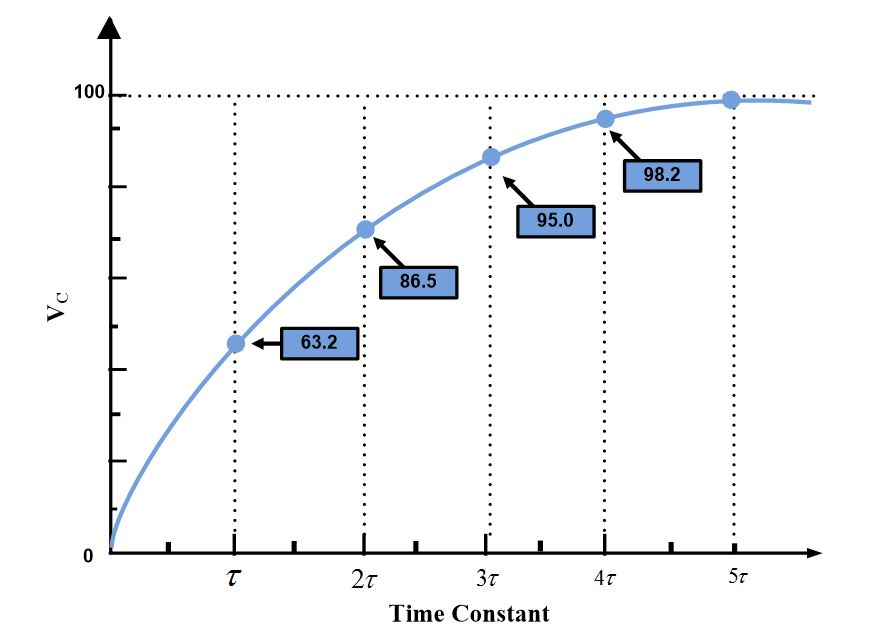
\includegraphics[width=225px]{\bank/ode/figures/tau_curve.jpg}
  \caption{Different values of capacitor voltage at different times, relative to $\tau.$}
  \label{fig:Tau Curve for Charging RC Circuit}
\end{figure}

\begin{enumerate}[resume]
\qitem OPTIONAL: On what order of magnitude of time (nanoseconds, milliseconds, 10's of seconds, etc.) does this circuit settle
($V_{\text{c}}$ is $>95\%$ of its value as $t \to \infty$)?

\sol{

The time constant $\tau$ of an RC circuit is just $\tau = RC$. For our circuit:
$$\tau = RC = \SI{100}{\ohm} \cdot \SI{10}{\micro\farad} = \SI{0.001}{\second} $$
After 3 time constants, the voltage will be $~95\%$ of its steady state value
$$3\tau = \SI{0.003}{\second}$$
The circuit will settle on the order of milliseconds.
Alternatively, this value can be found by using algebra:
$$0.95V_S = V_S(1 - e^{-\frac{t}{RC}}) $$
$$-0.05 = -e^{-\frac{t}{RC}} $$
$$0.05 = e^{-\frac{t}{RC}} $$
$$ln(0.05) = -\frac{t}{RC} $$
$$-3 = -\frac{t}{0.001} $$
$$t = 0.003 \, \text{seconds}$$
}

\meta{
	Students may be inclined to blindly use $\tau = RC$ to find a circuit's time constant, regardless of what the RC circuit looks like.
	Remind students that the time constant is only $RC$ for simple RC circuits with only one resistor and one capacitor, but it may be different for different circuits (for instance, the CMOS transistor models).
}

\qitem OPTIONAL: Give 2 ways to reduce the settling time of the circuit if we are allowed to change one component in the circuit.

\sol{

To reduce settling time, reduce $\tau$. We can achieve this by

\begin{enumerate}
\item Lowering the value of $R$ or
\item Lowering the value of $C$.
\end{enumerate}

Notice how the value of $V_{\text{s}}$ does not change the settling time.

}


\end{enumerate}
 % TODO: make this
\newpage

% THIS IS A PREVIEW QUESTION ON BOTH WORKSHEETS 1 AND 2
\qns{Multivariate ODE with Coordinate Changes}

\meta{
The general procedure for solving this type of problem is: First, convert to the eigenbasis. Solve the problem there. Then convert back to the problem basis to find the final answer.
}

\begin{enumerate}

\qitem Consider a system of differential equations (valid for $t\geq 0$)
\begin{equation}
\frac{d}{dt}x_1(t) = 5 x_1(t) + 2 x_2(t)
\end{equation}
\begin{equation}
\frac{d}{dt}x_2(t) = -8 x_1(t) -5 x_2(t)
\end{equation}

with initial conditions $x_1(0) = 3$ and $x_2(0) = 3$.

\textbf{Write out the differential equations and initial conditions in matrix/vector form.}

\ws{
	\vspace{120px}
}

\meta{
	When we say differential matrix, we're referring to a matrix that performs the act of differentation on the state variable $\vec{x}.$
}

\sol{
	We define our state variable $\vec{x}(t) = \begin{bmatrix}x_1(t) \\ x_2(t)\end{bmatrix}.$
	$$\ddt{}{t} \vec{x}(t) = \begin{bmatrix}\frac{d}{dt}x_1(t) \\ \frac{d}{dt}x_2(t)\end{bmatrix} = \begin{bmatrix}5 & 2 \\ -8 & -5\end{bmatrix}\begin{bmatrix}x_1(t) \\ x_2(t)\end{bmatrix} = \begin{bmatrix}5 & 2 \\ -8 & -5\end{bmatrix} \vec{x}(t)$$

	The initial condition is:
    $$\vec{x}(0) = \begin{bmatrix}x_1(0) \\ x_2(0)\end{bmatrix} =\begin{bmatrix}3 \\ 3\end{bmatrix} $$

    We will define the differential matrix as $A$, where

    $$A = \begin{bmatrix}5 & 2 \\ -8 & -5\end{bmatrix} $$
}

% \bigskip

% \begin{adjustwidth}{-20pt}{0pt}
% 	We already know how to solve the system of differential equations if $\frac{d}{dt}y_1(t)$ only depends on $y_1(t)$ and $\frac{d}{dt}y_2(t)$ only depends on $y_2(t)$.
% 	However, we can't directly solve a system of ODEs where $\frac{d}{dt}y_1(t)$ and $\frac{d}{dt}y_2(t)$ each depend on both $y_1(t)$ and $y_2(t)$. \\
% 	The solution? Change coordinates to the eigenbasis to diagonalize our transformation matrix.\\
% 	Then, we will have $\frac{d}{dt}z_{\lambda_1}(t) = \lambda_1 z_{\lambda_1}(t)$ and $\frac{d}{dt}z_{\lambda_2}(t) = \lambda_2 z_{\lambda_2}(t)$, which we know how to solve.

% \end{adjustwidth}


\qitem \textbf{Find the eigenvalues $\lambda_1, ~\lambda_2$ and eigenspaces for the differential equation matrix above.}

\ws{
	\vspace{150px}
}

\sol{
	In order to find the eigenvalues of $A,$ we look at the determinant of $A - \lambda I.$
	 $$\text{det}\left( \begin{bmatrix}5-\lambda & 2 \\ -8 & -5-\lambda\end{bmatrix} \right) = (-5-\lambda)(5-\lambda) + 16 = \lambda^2 - 9 = 0$$
	Therefore, we see that
	 $$ \lambda_1 = -3, \lambda_2 = 3$$

	We can find the eigenspaces by looking at the null-spaces of $A - \lambda I.$

	For $\lambda_1 = -3,$
	$$ (A + 3I) \vec v_{1}= \begin{bmatrix} 5 - (-3) & 2 \\ -8 & -5 - (-3) \end{bmatrix} \vec v_{1} = \begin{bmatrix}0 \\ 0\end{bmatrix}$$
    $$ \begin{bmatrix} 8 & 2 \\ -8 & -2 \end{bmatrix} \vec v_{1} = \begin{bmatrix}0 \\ 0\end{bmatrix}$$
    $$\vec v_{1} = \begin{bmatrix} -1 \\ 4\end{bmatrix} $$

	For $\lambda_1 = 3,$
	$$ (A - 3I) \vec v_{2} = \begin{bmatrix} 5 - 3 & 2 \\ -8 & -5 - 3 \end{bmatrix} \vec v_{\lambda_2} = \begin{bmatrix}0 \\ 0\end{bmatrix}$$
	$$ \begin{bmatrix} 2 & 2 \\ -8 & -8 \end{bmatrix} \vec v_{2} = \begin{bmatrix} 0 \\ 0\end{bmatrix}$$
	$$\vec v_{2} = \begin{bmatrix} -1 \\ 1\end{bmatrix} $$
}


\qitem
\textbf{Change coordinates into the eigenbasis to re-express the differential equations in terms of new variables $z_{1}(t), ~
z_{2}(t)$.}

Let $\vec{z}(t) = \begin{bmatrix} z_1(t) \\ z_2(t) \end{bmatrix}$ represent the vector $\vec{x}$ using the eigenbasis for its coordinate representation.
\textit{Find a matrix $\widetilde{A}$ such that $\frac{d}{dt} \vec{z}(t) = \widetilde{A} \vec{z}(t)$. Don't forget about the initial conditions.}

\ws{
	\vspace{200px}
}

\meta {
	$x_i$ coordinates are standard coordinates, while the $z_i$ coordinates are using the eigenbasis for representation.
}

\sol{
	\begin{centering}
	\begin{tikzpicture}

	\draw (-1,0) node[anchor = east] {$z_{i}$ coordinates};
	\draw (0,0) circle (0.5cm);
	\draw (-1,2) node[anchor = east] {$x_{i}$ coordinates};
	\draw[->] (0,0.5) -- (0,1.5) node[anchor=north east] {$V$};
	\draw (0,2) circle (0.5cm);
	\draw[->] (0.5,2) -- (4.5,2) node[anchor=south east] {$ A = \begin{bmatrix}5 & 2 \\ -8 & -5\end{bmatrix}$} ;
	\draw (3,2) node[anchor=north] {differentiation};
	\draw (5,2) circle (0.5cm);
	\draw[->] (5,1.5) -- (5,0.5) node[anchor=south west] {$V^{-1}$};
	\draw (5,0) circle (0.5cm);
	\draw[dashed,->] (0.5,0) -- (4.5,0) node[anchor=south east] {$ \widetilde{A} =V^{-1} A V$} ;

	\end{tikzpicture}
\end{centering}

$$\vec x = z_1 \vec v_{1} + z_2 \vec v_{2}$$
$$\vec x =\begin{bmatrix} -1 & -1 \\ 4 & 1\end{bmatrix}\begin{bmatrix}z_{1} \\ z_{2}\end{bmatrix}$$

We can define the change-of-coordinates matrix from the eigenbasis to our original basis as

$$V=\begin{bmatrix} -1 & -1 \\ 4 & 1\end{bmatrix}$$

Changing coordinates to the eigenbasis:

$$\begin{bmatrix}z_{1} \\ z_{2}\end{bmatrix} = V^{-1}\begin{bmatrix} x_1 \\ x_2\end{bmatrix}   $$

$$V^{-1}=\begin{bmatrix}\frac{1}{3} & \frac{1}{3} \\ -\frac{4}{3} & -\frac{1}{3}\end{bmatrix}$$

$$\widetilde{A} = V^{-1} A V = \begin{bmatrix}\frac{1}{3} & \frac{1}{3} \\ -\frac{4}{3} & -\frac{1}{3}\end{bmatrix}\begin{bmatrix}5 & 2 \\ -8 & -5\end{bmatrix}\begin{bmatrix} -1 & -1 \\ 4 & 1\end{bmatrix}$$
% $$A_{z_\lambda} = \begin{bmatrix}\frac{2}{3} & -\frac{1}{3} \\ \frac{1}{3} & \frac{1}{3}\end{bmatrix}\begin{bmatrix}-5 & -2 \\ 5 & -4\end{bmatrix}$$
$$\widetilde{A} = \begin{bmatrix}-3 & 0 \\ 0 & 3\end{bmatrix}$$

That is:

	$$\ddt{}{t} \vec{z}(t) = \begin{bmatrix}\frac{d}{dt} z_{1}(t) \\ \frac{d}{dt}z_{2}(t)\end{bmatrix} = \begin{bmatrix}-3 & 0 \\ 0 & 3\end{bmatrix}\begin{bmatrix}z_{1}(t) \\ z_{2}(t)\end{bmatrix}$$

And our initial condition is:

$$\vec z_{\lambda}(0) = \begin{bmatrix}\frac{1}{3} & \frac{1}{3} \\ -\frac{4}{3} & -\frac{1}{3}\end{bmatrix}\begin{bmatrix} 3 \\ 3 \end{bmatrix} = \begin{bmatrix} 2 \\ -5 \end{bmatrix} $$
}

\qitem \textbf{Solve the differential equation for $z_{1}(t)$, $z_{2}(t)$ in the eigenbasis.}

\ws{
	\vspace{150px}
}

\sol{
Our initial condition is $$\vec{z}(0) = \begin{bmatrix} 2 \\ -5 \end{bmatrix}$$

We can unroll our system of equations to get:

$$\ddt{}{t} z_{1}(t) = -3 z_{1}(t)$$
$$\ddt{}{t} z_{2}(t) = 3 z_{2}(t)$$

From previous differential equation experience, we see that the solution to $z_{i}(t)$ is:

$$z_{1}(t) = 2e^{-3t}$$
$$z_{2}(t) = -5e^{3t}$$
}

\qitem \textbf{Convert your solution back into the original coordinates to find $x_1(t)$, $x_2(t)$.}

\sol{
$$ \vec x(t) = V \vec z(t) =  \begin{bmatrix} -1 & -1 \\ 4 & 1\end{bmatrix}\begin{bmatrix} 2 e^{-3t} \\ -5 e^{3t}  \end{bmatrix} = \begin{bmatrix} -2e^{-3t} + 5 e^{3t}\\ 8e^{-3t}-5e^{3t} \end{bmatrix}$$
}


% \qitem We can solve this equation using a slightly shorter approach by observing that the solutions for $y_i(t)$ will all be of the form
% $$y_i(t) = \sum_k K_{i,k} e^{\lambda_k t}$$

% where $\lambda_k$ is an eigenvalue of our differential equation
% relation matrix and the $K_{i,k}$ are constants derived from our
% initial conditions and the coordinate changes involved.

% Since we have observed that the solutions will include
% $e^{\lambda_i t}$ terms, once we have found the eigenvalues for our
% differential equation matrix, we can guess the forms of the $y_i(t)$ as

%  	$$\begin{bmatrix}y_1(t) \\ y_2(t)\end{bmatrix}
%         = \begin{bmatrix}\alpha e^{\lambda_1t} + \beta e^{\lambda_2t}
%           \\ \gamma e^{\lambda_1 t}  + \kappa e^{\lambda_2 t} \end{bmatrix}$$
% where $\alpha, ~\beta, ~\gamma, ~\kappa$ are all constants.

% \begin{enumerate}
% 	\qitem Take the derivative to write out
% 	$$\begin{bmatrix}\frac{d}{dt}y_1(t) \\ \frac{d}{dt}y_2(t)\end{bmatrix}.$$ in matrix-vector form.

% 	\sol{
% 	 	$$\begin{bmatrix}y_1(t) \\ y_2(t)\end{bmatrix} = \begin{bmatrix}\alpha e^{-3t} + \beta e^{3t}  \\ \gamma e^{-3t}  + \kappa e^{3t} \end{bmatrix}$$
% 		$$\frac{d}{dt} \vec y(t) = \begin{bmatrix}-3\alpha e^{-3t} +3 \beta e^{3t}  \\ -3\gamma e^{-3t} + 3 \kappa e^{3t} \end{bmatrix}$$
% 		If we notice that the right-hand side can be written as linear combinations of $e^{-3t}$ and $e^{3t}$, we can write the previous equation as:
% 		$$ \frac{d}{dt} \vec y(t) =
% 		\begin{bmatrix}
% 			-3 \alpha & 3 \beta  \\ -3 \gamma & 3 \kappa
% 		\end{bmatrix}
% 		\begin{bmatrix}
% 			e^{-3t} \\ e^{3t}
% 		\end{bmatrix}
% 		$$
% 	}

% 	\qitem Connect this differential equation to the matrix-vector equation you found in part (a).\\
% 	\sol{
% 		$$\frac{d}{dt} \vec y(t) =
% 		\begin{bmatrix}
% 			5 & 2 \\
% 			-8 & -5
% 		\end{bmatrix}
% 		\vec{y}(t) =
% 		\begin{bmatrix}
% 			-3 \alpha & 3 \beta  \\ -3 \gamma & 3 \kappa
% 		\end{bmatrix}
% 		\begin{bmatrix}
% 			e^{-3t} \\ e^{3t}
% 		\end{bmatrix}
% 		$$
% 		Substituting
% 		$$ \begin{bmatrix}
% 			\alpha e^{-3t} + \beta e^{3t}  \\ \gamma e^{-3t}  + \kappa e^{3t}
% 		\end{bmatrix} =
% 		\begin{bmatrix}
% 			\alpha & \beta  \\ \gamma & \kappa
% 		\end{bmatrix}
% 		\begin{bmatrix}
% 			e^{-3t} \\ e^{3t}
% 		\end{bmatrix}
% 		$$
% 		for $\vec{y}(t)$, we get:
% 		$$
% 		\begin{bmatrix}
% 			5 & 2 \\
% 			-8 & -5
% 		\end{bmatrix}
% 		\begin{bmatrix}
% 			\alpha & \beta  \\ \gamma & \kappa
% 		\end{bmatrix}
% 		\begin{bmatrix}
% 			e^{-3t} \\ e^{3t}
% 		\end{bmatrix} =
% 		\begin{bmatrix}
% 			-3 \alpha & 3 \beta  \\ -3 \gamma & 3 \kappa
% 		\end{bmatrix}
% 		\begin{bmatrix}
% 			e^{-3t} \\ e^{3t}
% 		\end{bmatrix}
% 		$$
% 		Doing the matrix multiplication on the left-hand side of the equation, we get:
% 		$$
% 		\begin{bmatrix}
% 			5 \alpha + 2 \gamma & 5 \beta + 2 \kappa \\
% 			-8 \alpha - 5 \gamma & -8 \beta - 5 \kappa
% 		\end{bmatrix}
% 		\begin{bmatrix}
% 			e^{-3t} \\ e^{3t}
% 		\end{bmatrix} =
% 		\begin{bmatrix}
% 			-3 \alpha & 3 \beta  \\ -3 \gamma & 3 \kappa
% 		\end{bmatrix}
% 		\begin{bmatrix}
% 			e^{-3t} \\ e^{3t}
% 		\end{bmatrix}
% 		$$
% 	}

% 	\qitem Use what you found in the previous step to solve for $\gamma$ and $\kappa$ in terms of $\alpha$ and $\beta$, respectively. \\
% 	\sol {
% 		Equating terms in the matrices on the left- and right-hand sides of the equation, we get:
% 		$5 \alpha + 2 \gamma = -3 \alpha$,
% 		$5 \beta + 2 \kappa = 3 \beta$,
% 		$-8 \alpha - 5 \gamma = -3 \gamma$, and
% 		$-8 \beta - 5 \kappa = 3 \kappa$.

% 		From the first equation, we get $\gamma = -4 \alpha$. From the second, we get $\kappa = - \beta$. \\
% 		We could get the same result from using the third and fourth equations.
% 	}

% 	\qitem Use initial conditions to finish solving for $\vec{y}(t)$. \\
% 	\sol {
% 		From the initial condition, we have:
% 		$$\vec{y}(0) =
% 		\begin{bmatrix} 3 \\ 3 \end{bmatrix} =
% 		\begin{bmatrix}
% 			\alpha & \beta  \\ \gamma & \kappa
% 		\end{bmatrix}
% 		\begin{bmatrix}
% 			e^{-3 \cdot 0} \\ e^{3 \cdot 0}
% 		\end{bmatrix} =
% 		\begin{bmatrix}
% 			\alpha & \beta  \\ \-4 \alpha & - \beta
% 		\end{bmatrix}
% 		\begin{bmatrix}
% 			1 \\ 1
% 		\end{bmatrix}$$
% 		From this, we get the equations $\alpha + \beta = 3$ and $-4 \alpha - \beta = 3$.
% 		$$\alpha=-2$$
% 	 	$$\beta=5$$

% 		We can now plug in our 4 constants to find $\vec{y}(t)$:
% 		$$\begin{bmatrix}y_1(t) \\ y_2(t)\end{bmatrix} = \begin{bmatrix} -2e^{-3t} + 5e^{3t}  \\ 8e^{-3t}  -5  e^{3t} \end{bmatrix}$$
% 		Note that this is the same as the answer from part (e)
% 	}
% \end{enumerate}

\end{enumerate}
 % TODO: Fix up notation (replace z with x tilde)

\end{qunlist}

\end{document}
